\section{PLOT3 Plot 3D Function}

\subsection{Usage}

This is the 3D plot command.  The general syntax for its use is
\begin{verbatim}
  plot3(X,Y,Z,{linespec 1},X,Y,Z,{linespec 2},...,properties...)
\end{verbatim}
where \verb|X| \verb|Y| and \verb|Z| are the coordinates of the points on the
3D line.  Note that in general, all three should be vectors.  If
some or all of the quantities are matrices, then FreeMat will attempt
to expand the vector arguments to the same size, and then generate
multiple plots, one for each column of the matrices.  The linespec
is optional, see \verb|plot| for details.  You can specify \verb|properties|
for the generated line plots.  You can also specify a handle as an
axes to target
\begin{verbatim}
  plot3(handle,...)
\end{verbatim}
\subsection{Example}

Here is a simple example of a 3D helix.
\begin{verbatim}
--> t = linspace(0,5*pi,200);
--> x = cos(t); y = sin(t); z = t;
--> plot3(x,y,z);
Warning: Newly defined variable xlim shadows a function of the same name.  Use clear xlim to recover access to the function
Warning: Newly defined variable ylim shadows a function of the same name.  Use clear ylim to recover access to the function
Warning: Newly defined variable zlim shadows a function of the same name.  Use clear zlim to recover access to the function
--> view(3);
Warning: Newly defined variable xlim shadows a function of the same name.  Use clear xlim to recover access to the function
Warning: Newly defined variable ylim shadows a function of the same name.  Use clear ylim to recover access to the function
Warning: Newly defined variable zlim shadows a function of the same name.  Use clear zlim to recover access to the function
\end{verbatim}
Shown here


\centerline{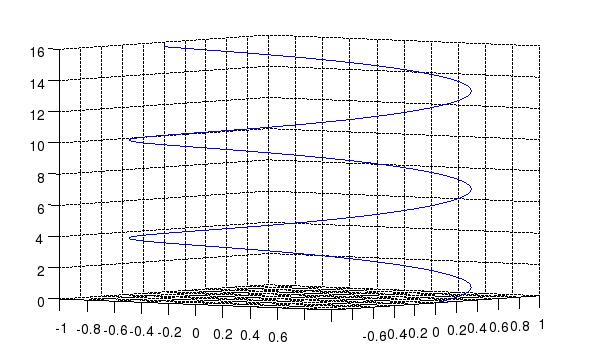
\includegraphics[width=8cm]{plt3}}

